%---------------------------------------------
%  CDUS QUADCHART TEMPLATE - 09/15/2025
%---------------------------------------------

\documentclass[aspectratio = 1610]{beamer}
\setbeamerfont{frametitle}{size=\tiny}
\setbeamerfont{caption}{size=\tiny}
\setbeamerfont{itemize/enumerate body}{size=\tiny}
\setbeamerfont{itemize/enumerate subbody}{size=\tiny}
\setbeamerfont{itemize/enumerate subsubbody}{size=\tiny}

\def\author{Hamza Mujtaba}

\newcommand{\FourQuad}[4]{
    \vspace{1em}
    \begin{columns}[c]
    \begin{column}{0.5\textwidth}
        \centering
        \vspace{-1em}
        \begin{minipage}[b][.453\textheight][t]{\textwidth}
            \vspace{5pt}
            #1
        \end{minipage} 
        \noindent\makebox[\linewidth]{\rule{0.48\paperwidth}{0.4pt}} 
        \begin{minipage}[b][.453\textheight][t]{\textwidth}
            \vspace{5pt}
            #3
        \end{minipage}
    \end{column}
    \hspace{-8pt}\vrule{}\hspace{8pt}
    \begin{column}{0.5\textwidth}
        \centering
        \vspace{-1em}
        \begin{minipage}[b][.453\textheight][t]{\textwidth}
            \vspace{5pt}
            #2
        \end{minipage} 
        \noindent\makebox[\linewidth]{\rule{0.48\paperwidth}{0.4pt}}
        \begin{minipage}[b][.453\textheight][t]{\textwidth}
            \vspace{5pt}
            #4
        \end{minipage}
    \end{column}
    \end{columns}
}

\newcommand{\quadrantTitle}[1]{ {\usebeamercolor[fg]{title} \tiny #1 }  \vspace{1mm} \\  }

\mode<presentation> {
    \usetheme{Malmoe}
    \usecolortheme[RGB={180,100,0}]{structure}
    \setbeamertemplate{items}[circle]
    \setbeamertemplate{navigation symbols}{} 
}

\usepackage{caption}
\usepackage{graphicx}
\usepackage[export]{adjustbox}
\usepackage{subcaption}
\usepackage{booktabs}

\begin{document}
\tiny
\begin{frame}{\author{} Quad Chart - May 5, 2026 }

\FourQuad%
{
    \quadrantTitle{ODAD Update}
    {\usebeamercolor[fg]{title} (1) Online adaptation development}
    \begin{itemize}
        \item \textbf{Top-k teacher selection} remains the best deployable ODAD branch.
        \item Track-aware/multi-track memory cleaned boxes but reduced detection.
        \item Stricter memory/geometry gates suppress valid target views.
        \item Next: checkpoint selection/rollback using online reliability proxies.
    \end{itemize}
}
{
    \quadrantTitle{Quantitative Ablation / Reliability}
    {\usebeamercolor[fg]{title} (2) Accuracy + error metrics on lab imagery}
    \vspace{0.3mm}
    \begin{center}
    \begingroup
    \tiny
    \setlength{\tabcolsep}{2.0pt}
    \renewcommand{\arraystretch}{1.05}
    \begin{tabular}{lccccc}
        \toprule
        Model & Det. & Weird & Jump & Bad & Good \\
        \midrule
        FDA-mix & \textbf{99.6\%} & 21.6\% & \textbf{2.0\%} & \textbf{15} & 97 \\
        Current ODAD & 96.8\% & 27.8\% & 10.6\% & 42 & 135 \\
        Multi-track & 93.2\% & 24.4\% & 8.0\% & 42 & \textbf{163} \\
        \bottomrule
    \end{tabular}
    \endgroup
    \end{center}
    \vspace{-2.2mm}
    {\tiny Streaks use ordered frames; Good = conf$\ge$0.25, no weird box/jump.}
    \vspace{-1.0mm}
    \begin{itemize}
        \item Multi-track improves symptoms but misses the 95\% detection target.
        \item Current ODAD remains the best deployable tradeoff.
        \item Streaks expose stability better than confidence alone.
    \end{itemize}
}
{
    \quadrantTitle{Lab Updates}
    {\usebeamercolor[fg]{title} (3) SSTI/Poster Updates}
    \begin{itemize}
        \item USSF Symposium poster drafted; awaiting final team review.
        \item Reliability tooling now writes summaries, streaks, and galleries.
        \item Next ODAD run: online checkpoint selection/rollback.
    \end{itemize}
}
{
    \quadrantTitle{Qualitative Reliability Examples}
    {\usebeamercolor[fg]{title} (4) ODAD vs FDA-mix galleries}\par
    \begin{minipage}{\linewidth}
    \centering
    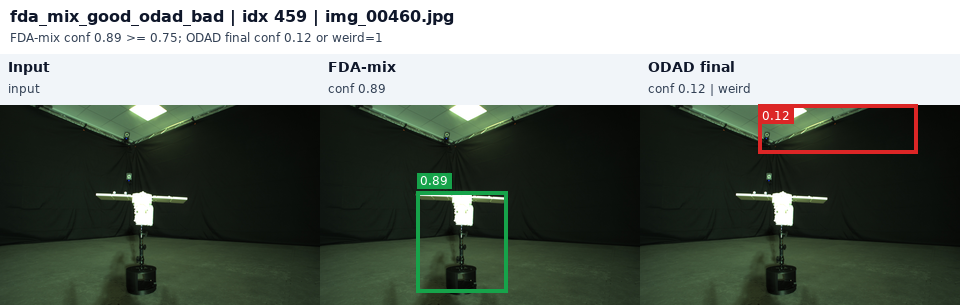
\includegraphics[width=0.98\linewidth,height=0.158\textheight,keepaspectratio]{odad_images/multitrack_fail_example.png}\\[-0.5mm]
    {\tiny FDA-mix good / Multi-track bad}\\[0.5mm]
    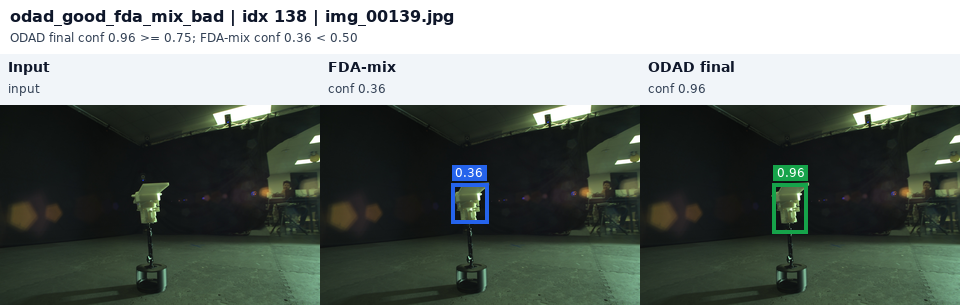
\includegraphics[width=0.98\linewidth,height=0.158\textheight,keepaspectratio]{odad_images/multitrack_success_example.png}\\[-0.5mm]
    {\tiny Multi-track good / FDA-mix weak}
    \end{minipage}
}
\end{frame}

\end{document}
